\documentclass[14pt]{extarticle}
\usepackage{fontspec}
\usepackage{polyglossia} % use instead of babel
\usepackage{pgfplots}
\usepackage{float}
\usepackage{amsmath}
\usepackage{amsfonts}
\setdefaultlanguage{hebrew}
\setotherlanguage{english}
\newfontfamily\hebrewfont[Script=Hebrew]{Arial}

% TODO: figure out if better to keep this or not, for word document pdf output similarity
\usepackage[margin=1in]{geometry}

% might be useful to ensure similarity to word document pdf output
% \usepackage{setspace}
% \singlespacing

% Reset equation counter at the start of each section
\usepackage{chngcntr}
\usepackage{etoolbox}
\counterwithin*{equation}{section}
\preto{\section}{\setcounter{equation}{0}}

% Left-aligned equation environment
\newenvironment{lefteqs}{%
    \begin{english}%
    \begin{flushleft}%
    \renewcommand{\arraystretch}{1.3}%
    $\begin{array}{@{}l@{}}%
}{%
    \end{array}$%
    \end{flushleft}%
    \end{english}%
}

\begin{document}

\begin{center}
    {\LARGE \textbf{מעבדה 1}}\\
    {\textbf{התאבכות בשכבות דקות}}
\end{center}

\begin{itemize}
    \item מגישים
    \begin{itemize}
        \item אורי כספי - 
        \item גיא גינזברג - 
        \item שי רואימי - 318986270
    \end{itemize}
    \item תאריך ביצוע הניסוי: 13 ביולי 2026
\end{itemize}
\newpage
\section*{ניסוי 2 - טבעות ניוטון}

\subsection*{מטרת הניסוי}

מדידת רדיוס העקמומיות $R$ של המשטח הקמור של עדשה מישורית-קמורה,
באמצעות תבנית ההתאבכות המתקבלת בטריז האוויר שבין העדשה ללוחית זכוכית שטוחה (טבעות ניוטון). המדידה מבוצעת עבור שלושה אורכי גל שונים.

\subsection*{רקע תיאורטי}

כשמניחים עדשה מישורית קמורה על זכוכית שטוחה נוצר ביניהן מרווח אוויר שעוביו
$d$
אפסי בנקודה בנקודה המגע, וגדל עם המרחק $r$ ממנה
הקשר בין $r$ ו $d$ הוא:
\begin{equation}
    R^2 = r^2 + (R - d)^2
\end{equation}

האיבר $d$ קטן מאוד ביחס ל $R$, ולכן ניתן להתעלם ממנו, ולקבל:
\begin{equation}
    d = \frac{r^2}{2R}
\end{equation}

כאשר:
\begin{itemize}
    \item $R$ - רדיוס העקמומיות של העדשה
    \item $r$ - המרחק מהנקודה בה נוצר המגע בין העדשה ללוחית הזכוכית
    \item $d$ - עובי שכבת האוויר בין העדשה ללוחית הזכוכית
\end{itemize}

האור המונוכרומטי הפוגע במרווח מוחזר גם מהמשטח התחתון של העדשה וגם מהמשטח העליון של הזכוכית, כאשר ההפרש הגיאומטרי בין הקרניים הוא $2d$

ההחזרה מהזכוכית (מעבר אוויר לזכוכית) גורם להפרש פאזה של $\pi$
וההחזרה מתחתית העדשה היא זכוכית לאוויר, ולכן אין תוספת בפאזה.

לכן התנאי להתאבכות הורסת הוא:

\begin{equation}
    2d + \frac{\lambda}{2} = (m + \frac{1}{2})\lambda \Rightarrow 2d = m\lambda
\end{equation}

כאשר:
\begin{itemize}
    \item $m$ - סדר הטבעות
    \item $\lambda$ - אורך הגל
\end{itemize}

הצבת (2) ב (3) נותנת את הקשר:
\begin{equation}
    r_m^2 = m \lambda R
\end{equation}

כאשר $r_m$ רדיוס הטבעת ה $m$.

\subsection*{מערכת המדידה ומהלך הניסוי}

הרכבנו את הרכיבים על ספסל אופטי בסדר הבא: ספק מתח, מנורת כספית,
מחזק מסננים, מתקן טבעות ניוטון, עדשה מרכזת, ומסך.

ראשית הרכבנו את המסנן הצהוב במחזק.

הזזנו את מחזק המסננים על המסילה עד שקיבלנו תמונה חדה של הטבעות,
ומדדנו את חמשת רדיוסי הטבעות הכהות הראשונות.
יש לציין שבמהלך המדידה החשכנו את החדר (כיבינו את האור וסגרנו את וילון הכניסה) על מנת שנוכל לראות את הטבעות על המסך.

המדידה נעשתה גם ויזואלית בהסתכלות ישירה על המסך, וכן ע"י צילום במכשיר טלפון והגברת הניגודיות במטרה לבצע מדידות מדויקות יותר.

לאחר מכן חזרנו על תהליך זה עבור המסנן הירוק והמסנן הסגול.

\subsection*{תוצאות וניתוח}

מצורפות תמונות של הטבעות על הלוחות:

\begin{figure}[H]
    \centering
    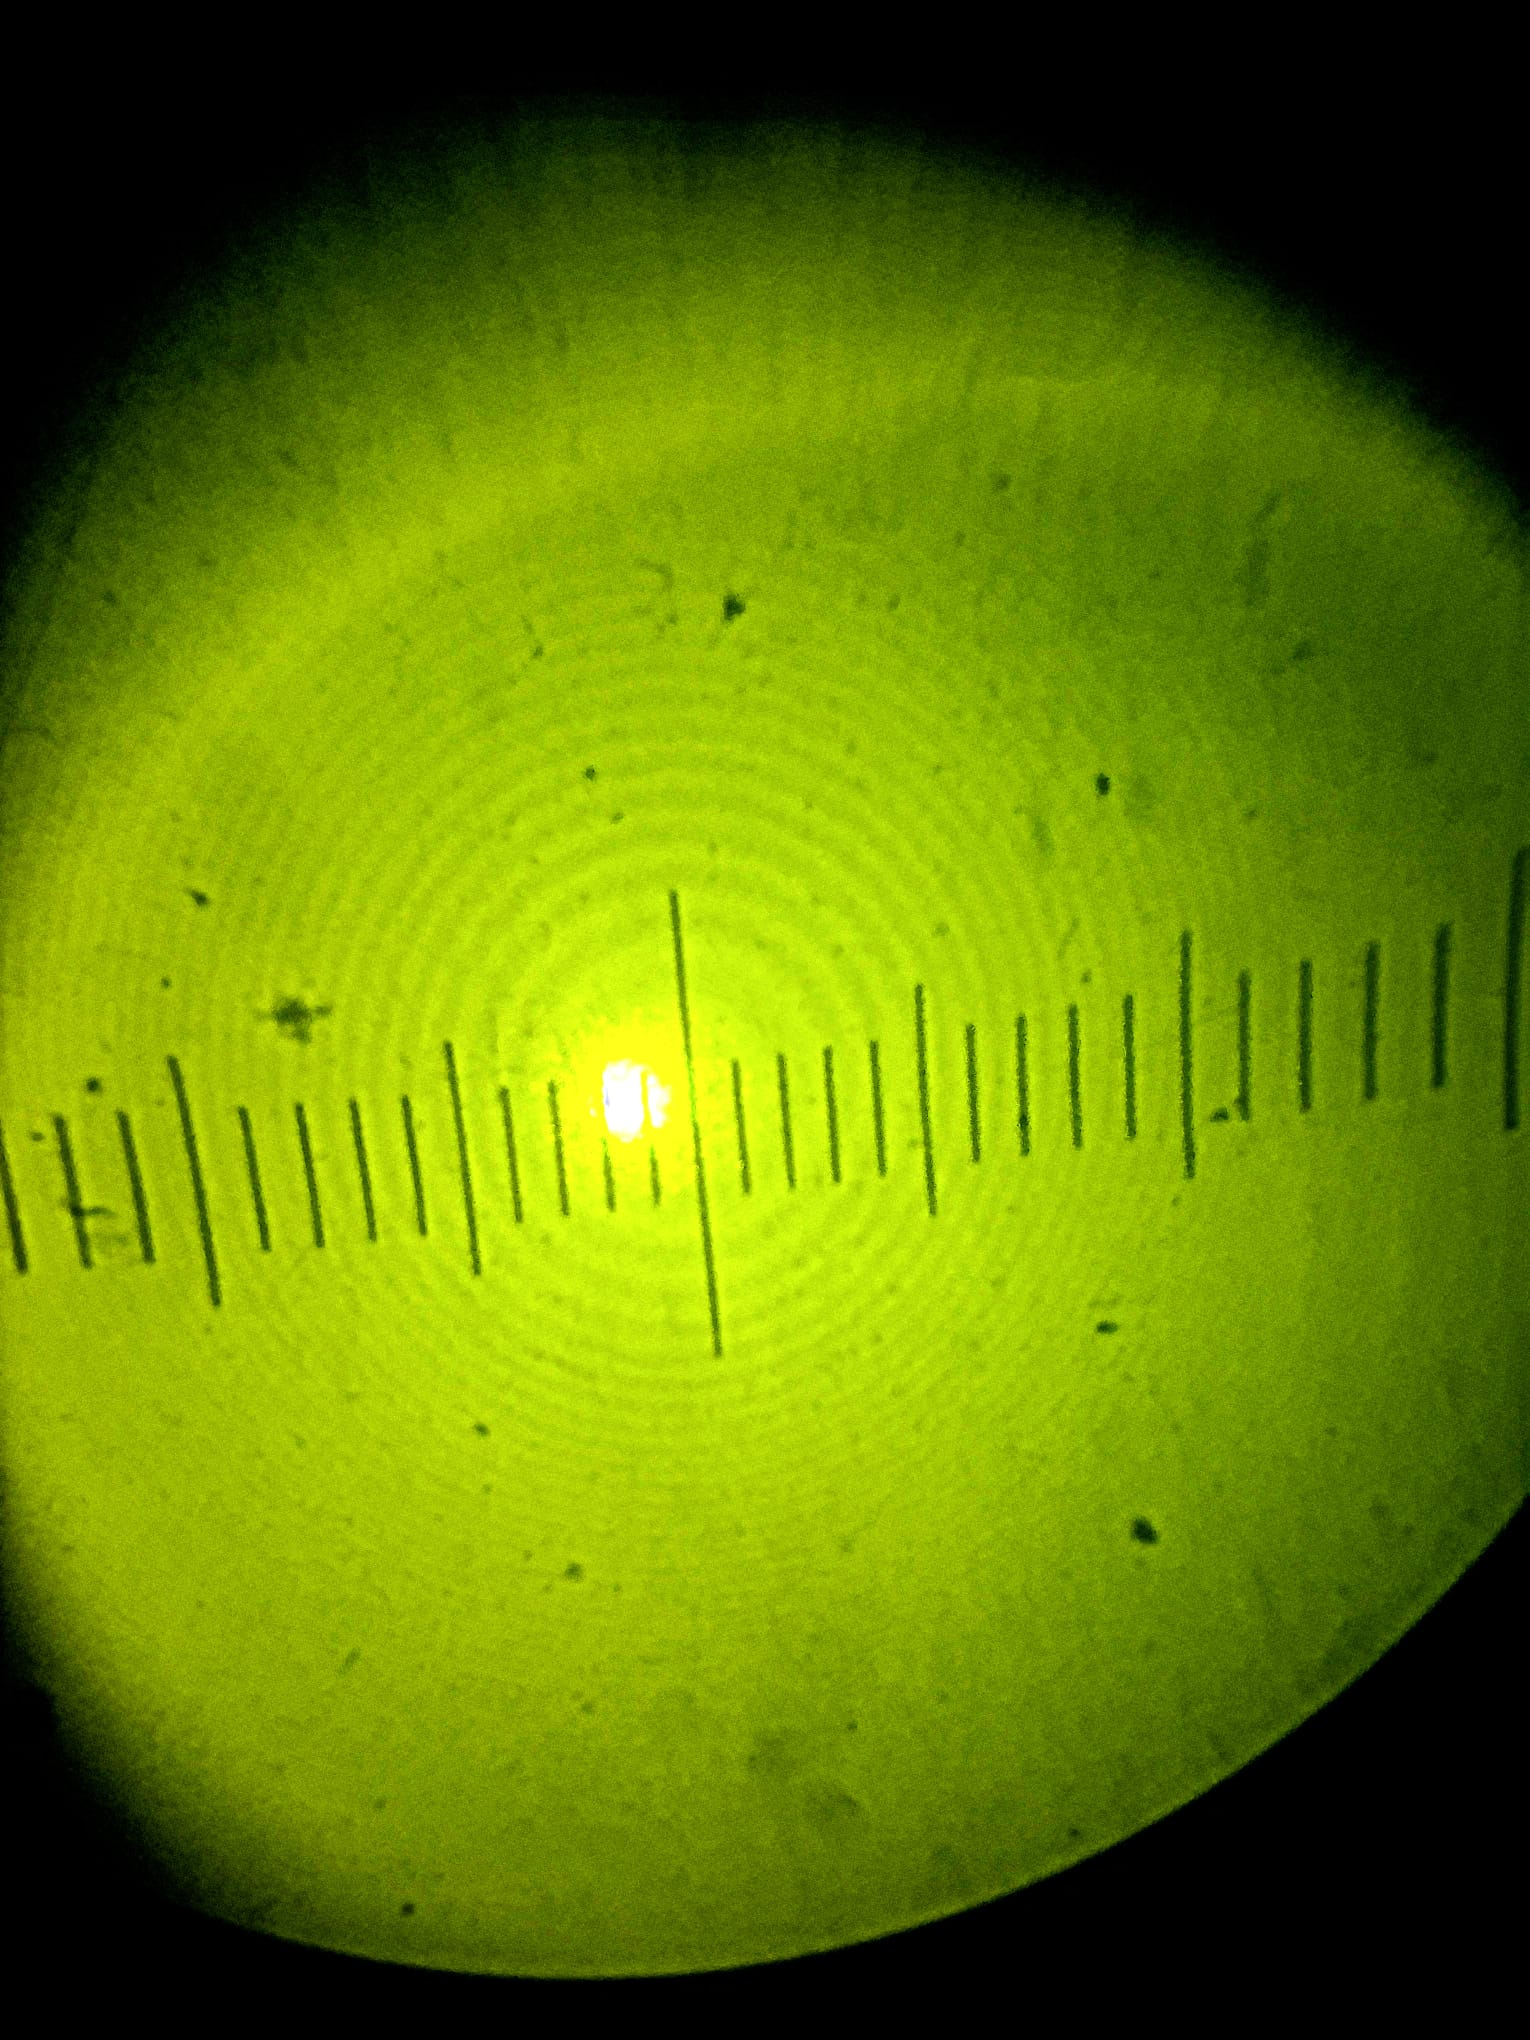
\includegraphics[width=0.8\textwidth]{L1E2_yellow_1.jpg}
    \caption{תמונה של טבעות ניוטון עם מסנן צהוב}
\end{figure}

\begin{figure}[H]
    \centering
    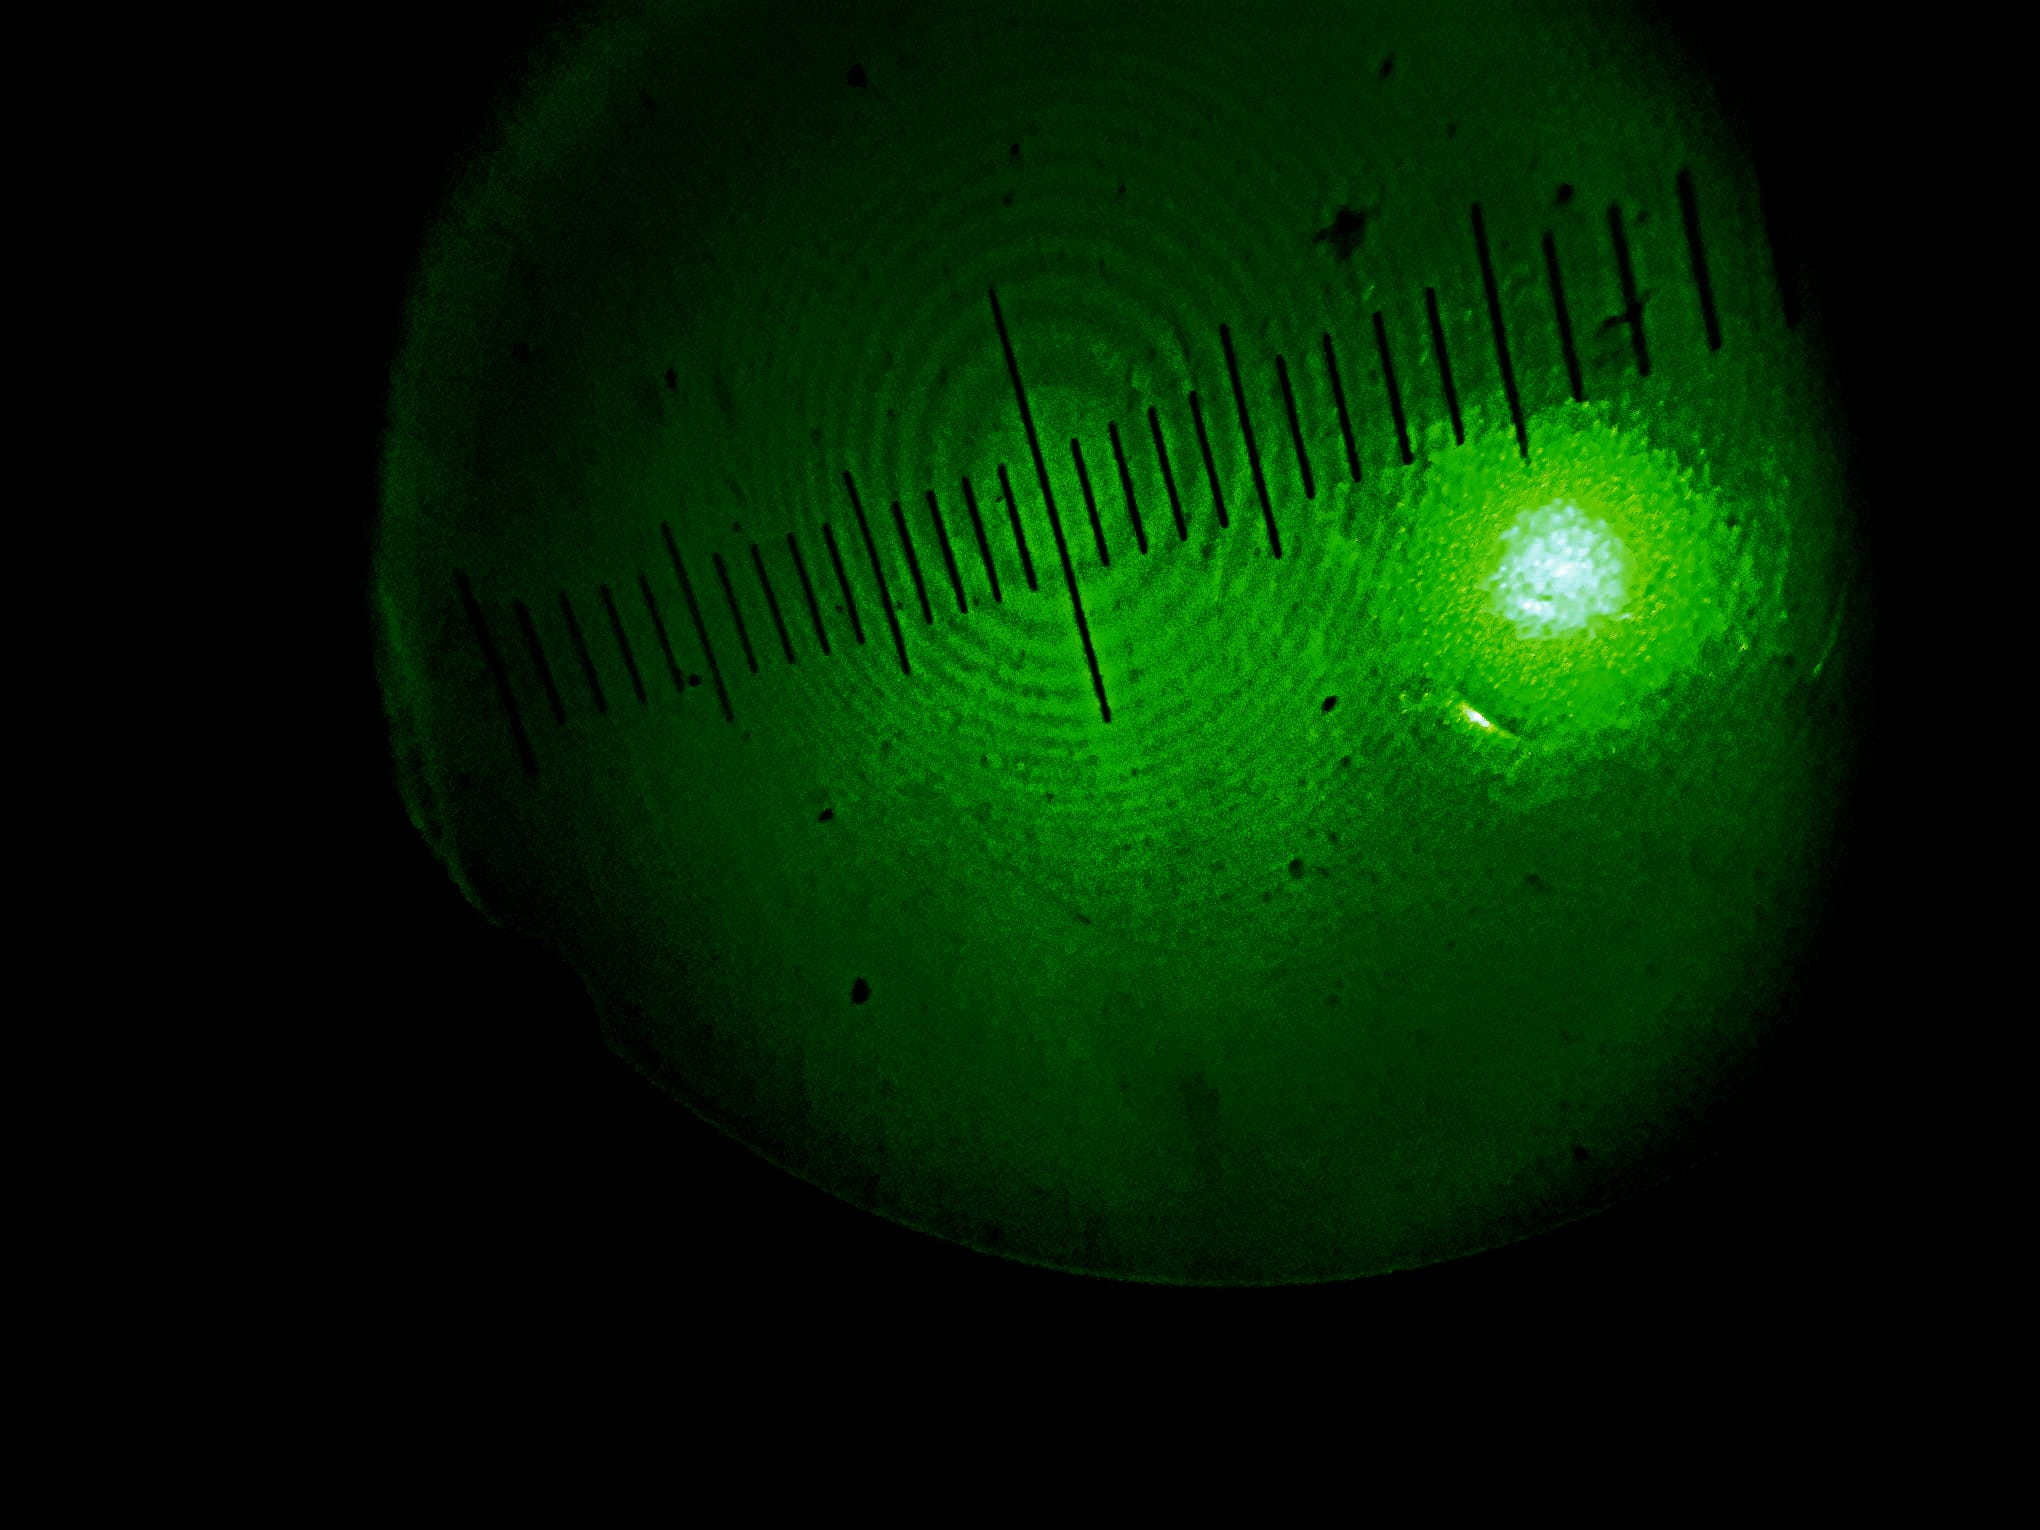
\includegraphics[width=0.8\textwidth]{L1E2_green_1.jpg}
    \caption{תמונה של טבעות ניוטון עם מסנן ירוק}
\end{figure}

\begin{figure}[H]
    \centering
    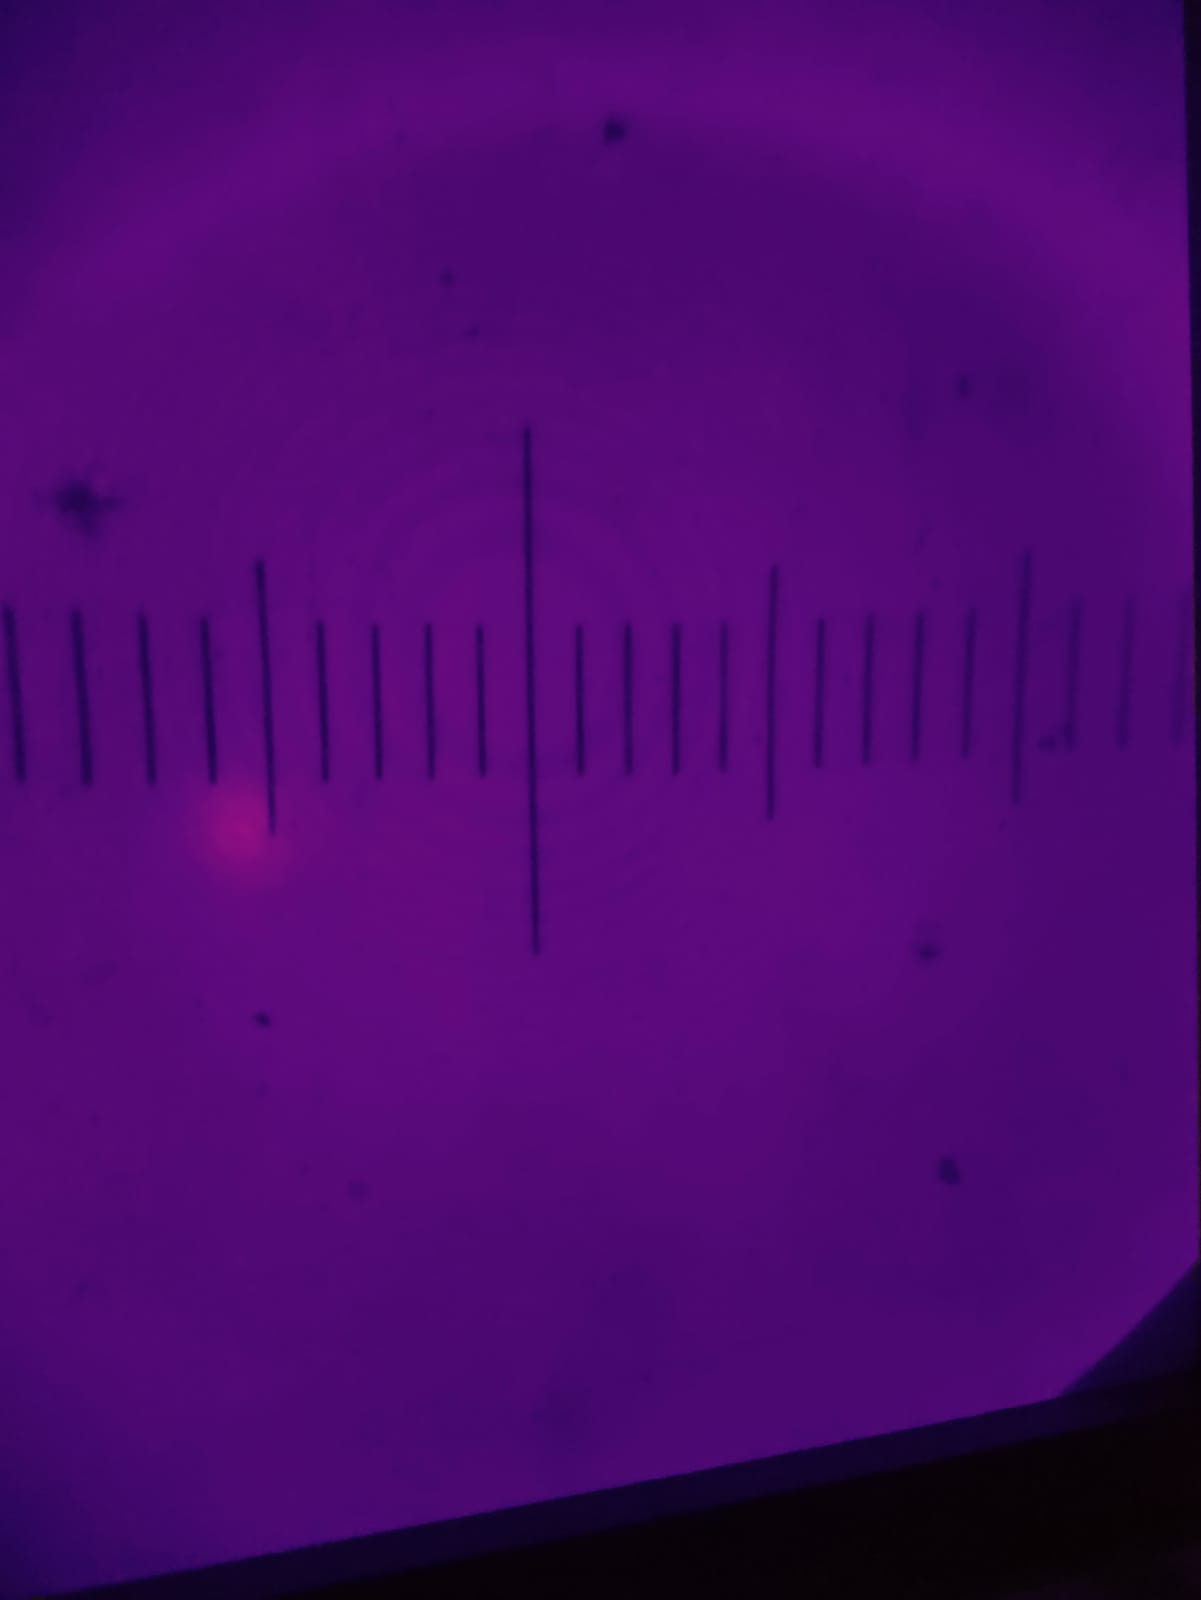
\includegraphics[width=0.8\textwidth]{L1E2_magenta_2.jpg}
    \caption{תמונה של טבעות ניוטון עם מסנן סגול}
\end{figure}

הרדיוסים שנמדדו לכל טבעת וריבועיהם כתובים בטבלאות הבאות, טבלה לכל מסנן.
ליד כל טבלה מצורפת תמונה של הגרף של $r_m^2$ כפונקציה של $m$, כאשר השיפוע של הגרף הוא $\lambda R$.

 עבור המסנן הצהוב:

\begin{table}[H]
    \centering
    \renewcommand{\arraystretch}{1.5} % Increase row height
    \begin{tabular}{|c|c|c|}
        \hline
        \text{[$mm^2$] $r_m^2$} &\text{[mm] $r_m$}& \text{$m$} \\ \hline
        6.2 & 2.5 & 1 \\ \hline
        11.6 & 3.4 & 2 \\ \hline
        17.7 & 4.2 & 3 \\ \hline
        25 & 5.0 & 4 \\ \hline
        31.4 & 5.6 & 5 \\ \hline
    \end{tabular}
    \caption{מסנן צהוב}
    \label{tab:newton_rings_yellow}
\end{table}

\begin{figure}[H]
    \centering
    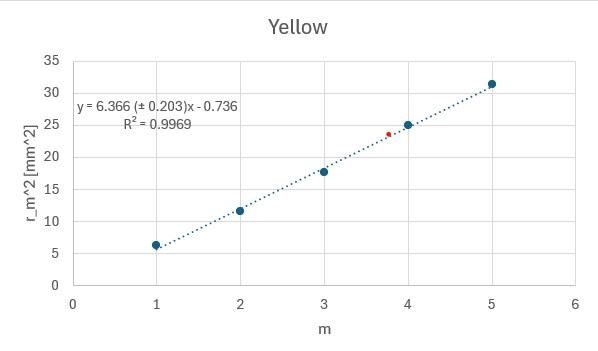
\includegraphics[width=0.8\textwidth]{L1E2_yellow_graph.jpg}
    \caption{גרף של $r_m^2$ כפונקציה של $m$ עבור המסנן הצהוב}
\end{figure}

 עבור המסנן הירוק:

\begin{table}[H]
    \centering
    \renewcommand{\arraystretch}{1.5} % Increase row height
    \begin{tabular}{|c|c|c|}
        \hline
        \text{[$mm^2$] $r_m^2$} &\text{[mm] $r_m$}& \text{$m$} \\ \hline
        4.8 & 2.2 & 1 \\ \hline
        9.6 & 3.1 & 2 \\ \hline
        16 & 4 & 3 \\ \hline
        23 & 4.8 & 4 \\ \hline
        27 & 5.2 & 5 \\ \hline
    \end{tabular}
    \caption{מסנן ירוק}
    \label{tab:newton_rings_green}
\end{table}

\begin{figure}[H]
    \centering
    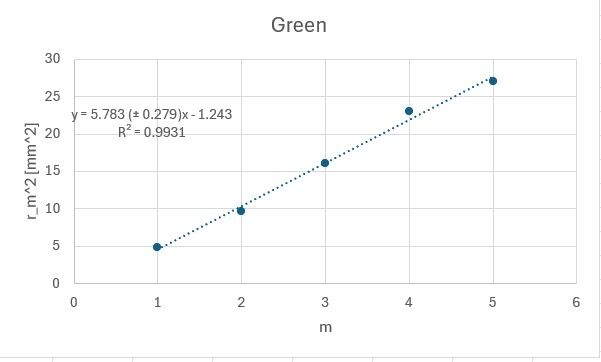
\includegraphics[width=0.8\textwidth]{L1E2_green_graph.jpg}
    \caption{גרף של $r_m^2$ כפונקציה של $m$ עבור המסנן הירוק}
\end{figure}

 עבור המסנן הסגול:

\begin{table}[H]
    \centering
    \renewcommand{\arraystretch}{1.5} % Increase row height
    \begin{tabular}{|c|c|c|}
        \hline
        \text{[$mm^2$] $r_m^2$} &\text{[mm] $r_m$}& \text{$m$} \\ \hline
        5.3 & 2.3 & 1 \\ \hline
        10.2 & 3.2 & 2 \\ \hline
        16.8 & 4.1 & 3 \\ \hline
        23 & 4.8 & 4 \\ \hline
        28 & 5.2 & 5 \\ \hline
    \end{tabular}
    \caption{מסנן סגול}
    \label{tab:newton_rings_purple}
\end{table}

\begin{figure}[H]
    \centering
    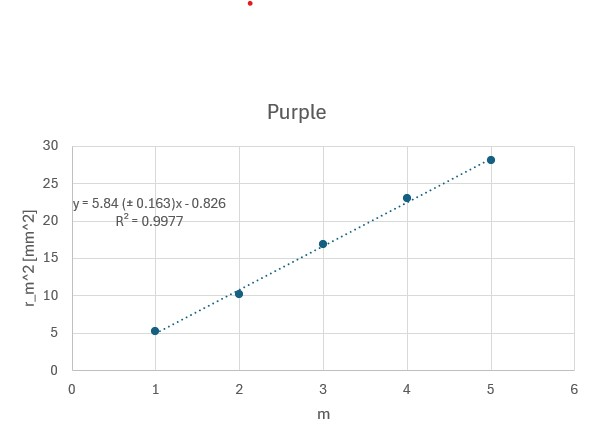
\includegraphics[width=0.8\textwidth]{L1E2_purple_graph.jpg}
    \caption{גרף של $r_m^2$ כפונקציה של $m$ עבור המסנן הסגול}
\end{figure}

ע"י הצבה של שיפוע הגרף בנוסחא (4) ניתן לחשב את רדיוס העקמומיות של העדשה עבור כל מסנן.

את שגיאת שיפוע קו המגמה נחשב בעזרת LINEST

במדידה במסנן הצהוב התקבל שיפוע של $6.366$, כלומר רדיוס העקמויות של העדשה  והשגיאה מהגרף הם:

\begin{lefteqs}
    R = \frac{6.366}{\lambda_{yellow}} = \frac{6.366}{0.578} = 11.01 mm \\
    \Delta R = \frac{0.203}{0.578} = 0.34 mm
\end{lefteqs}

במדידה במסנן הירוק התקבל שיפוע של $5.783$, כלומר רדיוס העקמויות של העדשה והשגיאה מהגרף הם:
\begin{lefteqs}
    R = \frac{5.783}{\lambda_{green}} = \frac{5.783}{0.546} = 10.59 mm \\
    \Delta R = \frac{0.279}{0.546} = 0.51 mm
\end{lefteqs}

במדידה במסנן הסגול התקבל שיפוע של $5.84$, כלומר רדיוס העקמויות של העדשה והשגיאה מהגרף הם:
\begin{lefteqs}
    R = \frac{5.84}{\lambda_{purple}} = \frac{5.84}{0.436} = 13.39 mm \\
    \Delta R = \frac{0.163}{0.436} = 0.37 mm
\end{lefteqs}

ערכו הממוצע של $R$ הוא:

\begin{lefteqs}
    R_{avg} = \frac{11.01 + 10.59 + 13.39}{3} = 11.66 mm
\end{lefteqs}

את שגיאת המדידת הכוללת נרכיב מהשגיאה הסטטיסטית משלושת המסננים ומשגיאת המדידה עבור כל מסנן.

השגיאה הסטטיסטית היא (ע"פ נוסחא 2 בפרק שגיאות מדידה):

\begin{lefteqs}
    \Delta R_{statistical} = \sqrt{\frac{(11.01 - 11.66)^2 + (10.59 - 11.66)^2 + (13.39 - 11.66)^2}{3}} = 1.23 mm
\end{lefteqs}

שגיאת המדידה היא:

\begin{lefteqs}
    \Delta R_{measurement} = \frac{\sqrt{0.34^2 + 0.51^2 + 0.37^2}}{3} = 0.29 mm
\end{lefteqs}

השגיאה הכוללת היא:

\begin{lefteqs}
    \Delta R_{total} = \sqrt{(1.23)^2 + (0.29)^2} = 1.26 mm
\end{lefteqs}

כלומר:

\begin{lefteqs}
    R = 11.66 \pm 1.26 mm
\end{lefteqs}

השגיאה היחסית ביחס לנתוני היצרן $(12 mm)$ היא:

\begin{lefteqs}
    \frac{|R_{avg} - R_{ref}|}{R_{ref}} = \frac{|11.66 - 12|}{12} \approx 2.83\%
\end{lefteqs}

\end{document}
